% Copyright (c) 2014,2016 Casper Ti. Vector
% Public domain.

\chapter{利用CNN分辨NLDBD事件和背景事件}
\label{chapter:cnn}

正如上文所述,NLDBD事件是一个及其稀有的事件,其半衰期超过了$1.07\times10^{26}$年,因而对于实验中的本底控制提出了很高的要求。根据第\ref{chapter:background}章所进行的背景模拟数据,PandaXIII实验中200kg级的探测器每年会探测到约78个本底$\gamma$事件落在ROI能量区间中,这个事件率还是远远高于实验的需求,因而需要一些其他的方式来压低本地信号,其中最自然的方法便是利用事件径迹的相关信息来区分背景事件和NLDBD事件。

NLDBD事件会同时释放出两个高能电子,在其径迹的两个末端会有这十分明显的布拉格峰,这是NLDBD事件最为明显的一个特征。而传统的$\gamma$本底事件一般通过一次或多次康普顿散射产生一个或多个次级电子,所以$\gamma$射线的径迹会形成一个或多个单末端布拉格峰的径迹。所以如果我们能够得到探测器探测到事件的详细径迹信息,就可以由此高效的分辨出本底事件和NLDBD事件,从而极大的压低本地。

然而因为PandaXIII读出系统的限制,使用传统的方法重建径迹会变得比较困难,因而我们探究了使用CNN深度神经网络来进行事件鉴别这一方法,得到了较为优异的效果。本章节详细描述了利用CNN进行事件鉴别的动机,CNN模型的选择和搭建,数据处理和训练等细节,希望能够帮助读者建立起对于CNN清晰简单的认识,为高能物理研究甚至是其他领域的研究提供相应的帮助。

\section{传统鉴别方法以及遇到的困难}

如前文所述,NLDBD是一个径迹特征即为明显的事件,该特征能够极大地帮助实验的进行。图\ref{fig:samples}给出了NLDBD和背景事件的对比,可以很明显的看出NLDBD事件径迹在末端拥有两个明显的布拉格峰,而背景$\gamma$事件则只存在一个布拉格峰。如果我们的TPC能够完美的重建出事件的径迹信息,那么鉴别该事件是否是NLDBD事件就会变得及其的简单:我们只要重建出径迹沉积的能量随径迹位置的关系,然后使用简单的cut就可以判断该事件的类型。然而在PandaXIII中重建径迹这个操作是十分困难的,原因如下。

\begin{figure}[hbt]
    \centering
    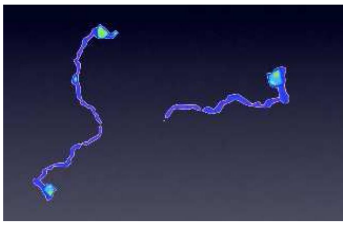
\includegraphics[width=0.5\columnwidth]{pic/fig10.png}
    \caption{一个NLDBD事件(左图)和一个$\gamma$背景事件(右图)径迹投影图。可以很明显的分辨出左侧径迹末端有两个布拉格峰,而右侧只有一个末端有布拉格峰。}
    \label{fig:samples}
\end{figure}

PandaXIII设计使用了41个Microbulk Micromegas读出板来构建读出平面,每个MM(Microbulk Micromegas)板的尺寸为20厘米x20厘米,按照图\ref{fig:mms}所示的形状排列组成,这样的话读出平面能够极大的覆盖漂移区域,从而提升事件的探测效率。

\begin{figure}[hbt]
    \centering
    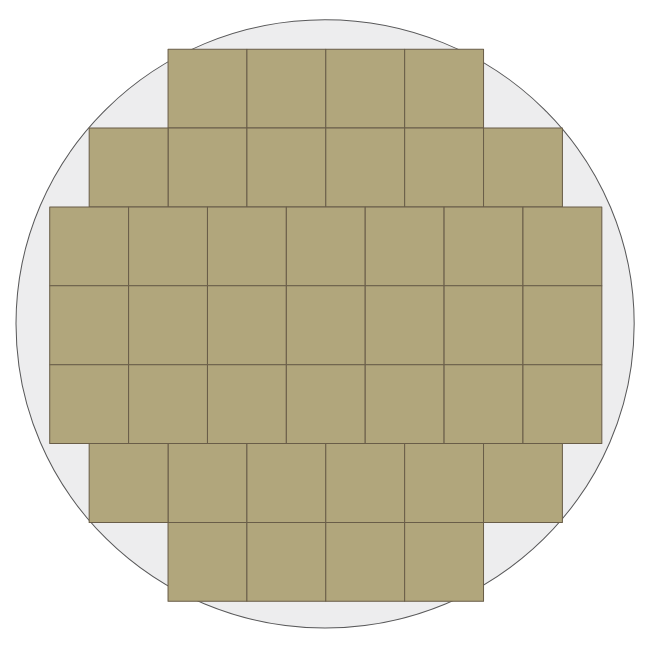
\includegraphics[width=0.4\columnwidth]{pic/fig8.png}
    \caption{41个MM板组合探测器读出平面排放示意图,按照4,6,7,7,7,6,4层叠放置。}
    \label{fig:mms}
\end{figure}

如图\ref{fig:mm_detail}左图所示,每个MM上都密布了许多增益孔(Amplification holes),用于采集漂移到附近的电子。这些增益孔按照合适的排布组成菱形的读出像素,每个像素的对角线尺寸约为3毫米,这边是Micromegas的位置分辨率。如果MM采取像素读出的话,一块MM会拥有约4000个通道(channel),整个TPC则会超过32万,这么多道数对于电子学部分基本是不可以承受的,因而PandaXIII使用了条状读出,而不是像素读出。如图\ref{fig:mm_detail}右图所示,每一组红色像素被连接在一起,在Y方向上形成64个通道,X方向上同样由黄色像素组成64个通道。这样的话一块MM读出板只会形成128个通道,从而大大降低了电子学的复杂程度。

\begin{figure}
    \centering
    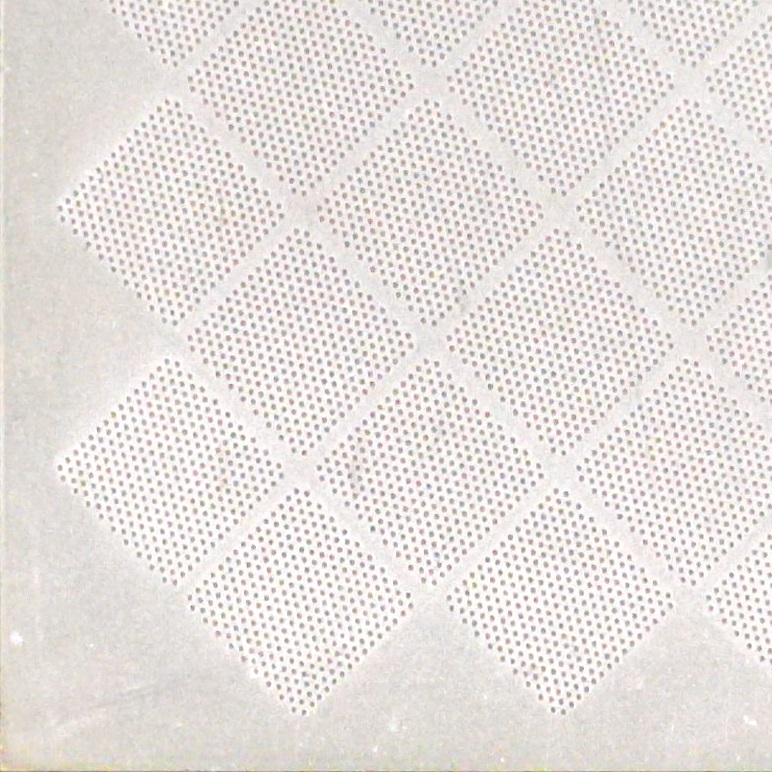
\includegraphics[width=0.4\columnwidth]{pic/MMStrips.jpg}
    \includegraphics[width=0.4\columnwidth]{pic/MMPattern.pdf}
    \caption{左图,MM板局部读出区域的放大示意图,图中的小孔便是增益孔(Amplification Holes),若干孔组成一个菱形读出像素,每个像素的对角线长度约为3毫米。右图:MM板局部读出通道(channel)连接示意图,红色以及黄色菱形(正方形)区域即为中图所示的读出像素,每一条红色虚线或者黄色虚线连接了一组读出像素,形成一个读出通道。\supercite{lin2018design}}
    \label{fig:mm_detail}
\end{figure}

但是采取条状读出也有对应的弊端,即我们无法同时获取到漂移到MM读出板上电子的X和Y的位置,我们只能得到它的X\textbf{或}Y的位置。再加上通过漂移时间计算得到的Z轴相对位置关系后,我们能够轻易的得到一个事件的X-Z-energy投影信息和Y-Z-energy投影信息,而有关X-Y的信息则因为MM结构问题而被彻底抹去了,这就使得重建径迹的3维信息变得极其的困难。

虽然一条比较直的径迹可以紧紧通过X-Z以及Y-Z来组合得到X-Y-Z的径迹,但是电子在TPC中的运动径迹往往不规则,同一时刻往往会有超过一组X和Y读出条被触发,这样同一Z值(同一时刻)的XY信息就无法确定,如图\ref{fig:difficulty_track_2}所示。如果两个真实的hit分别位于($x_1$,$y_1$)和($x_2$,$y_2$),那么因为条状读出的原因,$x_1,x_2,y_1,y_2$所在的通道会同时被触发,那么重建就可能得到错误的能量沉积点。图\ref{fig:difficulty_track}便给出了一个难于重建的
NLDBD事件投影图,该事件在Z在(80,110)毫米处的径迹纠缠在了一起,所以基本上不可能完成重建。

\begin{figure}
    \centering
    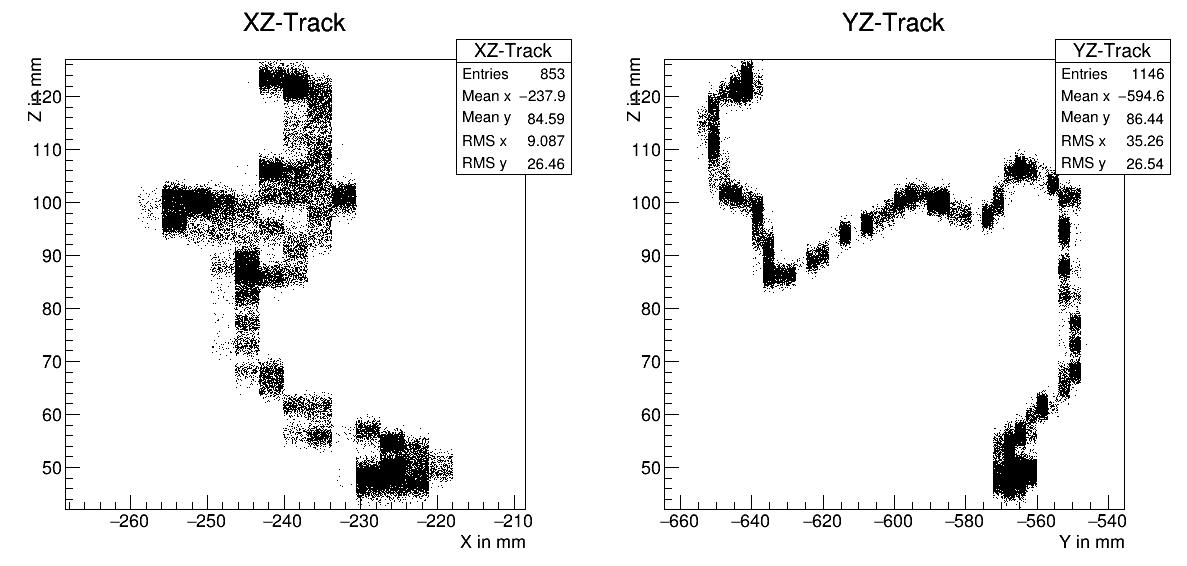
\includegraphics[width=0.7\columnwidth]{pic/difficulty_track.png}
    \caption{一个难于重建的事件的XZ投影和YZ投影,区块深浅表示沉积能量的大小,Z在(80,110)毫米内的径迹因为X方向上的多种可能而变得无法重建。}
    \label{fig:difficulty_track}
\end{figure}

\begin{figure}
    \centering
    \includegraphics[width=0.4\columnwidth]{pic/app01_strip_readout.pdf}
    \caption{条状读出易混淆的示意图。真实的能量沉积位置如图中绿色点所示($x_1$,$y_1$)和($x_2$,$y_2$),但是因为$x_1,x_2,y_1,y_2$所在的通道同时被触发,因而可能得到红色表示的错误重建结果。}
    \label{fig:difficulty_track_2}
\end{figure}

MM条状读出同时还带来了另外一个困难,因为一个电子要么落在X读出条所在的像素中,要么落在Y读出条所在的像素中,因而径迹相同位置在重建后的两个投影处的能量并不相等。所以根据能量的大小做X-Y的匹配也困难重重。作者个人认为在使用MM条状读出的前提下,能够良好的重建出径迹基本是不可能的,因而需要探寻新型的事件鉴别的方式方法。于是我们便试图将近年来在计算机领域大放异彩的深度神经网络引入我们的粒子鉴别,以期望它能够解决这个难题。

\section{CNN介绍以及使用动机}

\subsection{使用动机}
正如上文所说的,使用MM作为读出时很难通过重建出3维径迹后利用物理图像直接分类,但是如果将形如图\ref{fig:samples}的图片交于人眼来识别,那么相信绝大部分的人都可以轻而易举的分辨出NLDBD事件和背景$\gamma$事件。同时在这个分辨过程中我们并没有试图将两个偷影重建成3维的信息,而是直接通过分析比较两个投影并找到径迹的末端。这种行为操作相对来说难于量化,虽然可能可以通过精细的CUT达成,但是在这些操作的过程中可能需要人工的丢掉大量的数据以降低CUT的复杂度,这都不是我们所希望的。

近些年来随着机器学习技术的快速发展,我们发现似乎CNN真的能够进行一些类似于人类智能的处理,例如Google公司所开发的围棋AI,AlphaGo\supercite{gibney2016google},更是击败了诸多现役棋手,本文会在下一小节详细介绍有关机器学习和CNN的知识。鉴于CNN如此“智能“的表现,我们希望它能够完成类似自然人所做到的事情,即通过观察径迹的两个方向上的投影而做出事件类型的判断。而事实上CNN也较为完美的达到了我们的目标,有关测试的结果见章节\ref{section:cnn_result}。

\subsection{神经网络介绍}

关于神经网络的介绍最早应该从机器学习开始。人们一直在探寻人类自身智慧的来源,从一开始的哲学方面的探讨,再到近代从生物学医学的方向出发,智能一直是科学界中最令人着迷的一个方向。在1949年加拿大心理学家唐纳德·赫布提出了赫布理论\supercite{hebbian},为生物神经网络的学习做出了理论的支撑。1952年IBM的Arthur Samuel开发了一个国际跳棋程序,他发现他构造的这个程序能够随着局数的增多而下得越来越好,因而他给出了机器学习最初的定义,即”不需要显式编程就可以赋予机器某项能力的研究领域“。随后的几十年,机器学习领域一直在慢慢的发展,也分化除了若干个方向,包括1986年由J. R. Quinlan提出的决策树,1995年Vapnik和Cortes提出的支持向量机(Support Vector Machine,SVM)等\supercite{mlhistory}。直到2008年后,英伟达公司所提出的统一计算构架(Compute Unified Device Architecture,CUDA)\supercite{CUDA}的出现,人们利用计算机能够得到的计算能力极大地增强,机器学习中沉寂了许多年的神经网络方向才得以快速的发展,重新回到了大众的视线。

无论是递归神经网络(Recurrent Neural Network, RNN),卷积神经网络 
(Convolutional Neural Network,CNN),抑或是对抗神经网络
(Generative Adversarial Network,GAN),他们都离不开神经网络(Neural Network),神经网络最基本的组织单元便被称为神经元(Neural)。每一个神经元都拥有着若干个输入,并通过一定的算法将这些输入和自身存储的参数一起进行处理,给出一个或多个输出。简单而言,对于一组输入$(x_1,x_2,...,x_n)$,单输出的神经元为:
$$ y= f(x_1,x_2,...x_n,a_1,a_2,...,a_m)$$
其中$(a_1,a_2,...,a_n)$是神经元自身的参数,f为某一种非线性函数。当然实际上我们使用的神经元的结构相对简单,一个显著的全连接神经网络中的神经元如下所示:
\begin{equation}
     y=g(\omega_1 x_1+\omega_2 x_2 + ... + \omega_n x_n+ \omega_0))
     \label{eq:neural}
\end{equation}
其中$(\omega_1,\omega_2,...,\omega_n)$被称作权重,$\omega_0$为偏置(Bias),$g(z)$则被成为激活函数(Activation Function),它的主要作用是提供一个非线性的部分。一个典型的被称作sigmod的激活函数表达形式为:
$$g(z)=\frac{1}{1+e^{-z}}$$
显然,一个神经元的输出可以当做另外一个神经元的输入,许多神经元共同组成一个网络,像自然中的神经细胞一样相互影响,共同对输入量做出反应,这就是一个神经网络。然而为了简化模型,我们通常会对网络进行分层研究。

当若干个相似的神经元共同对一组输入做出反应时,我们可以将其称之为一层网络,即$\bar Y = F( \bar X, \omega_1,...,\omega_n)$
其中输入便是一个张量(tensor)$\bar X$,输出则是另外一个张量$\bar Y$。许多不同类型的层相互层叠,每一层的输出作为下一层的输入,最终形成一个
\begin{equation}
    \bar Y_0 = \mathcal{F}(\bar X_0, \mathcal{W})
\end{equation}的非线性系统。而神经网络的训练便是寻找最能够拟合已知输入输出的参数们$\mathcal{W}$。图\ref{fig:simple_nn}展示了一个简单的全连接神经网络示意图,该网络接受一个维度(shape)为(3)的张量作为输入,并输出一个维度为(1)的张量(标量)。

\begin{figure}
    \centering
    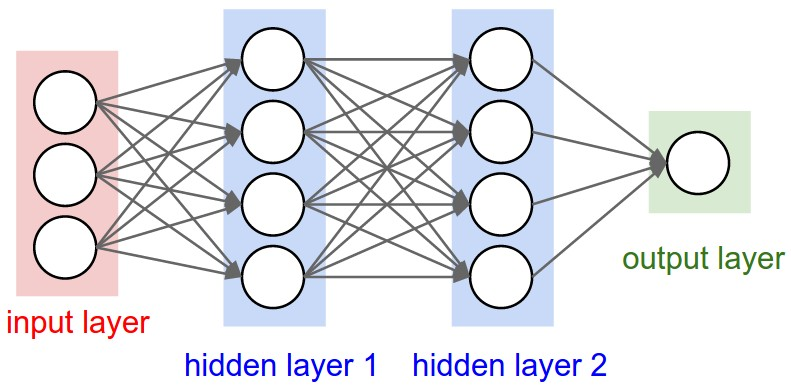
\includegraphics[width=0.7\columnwidth]{pic/simple_nn.jpeg}
    \caption{一个简易的全连接神经网络,包含一个输入层,两个隐含层以及一个输出层。}
    \label{fig:simple_nn}
\end{figure}

一个神经网络中所有神经元的参数便被成为这个网络的权重(Weight),而神经网络中的层的类型和层的属性(神经元数目,组合方式)则被称作模型(Model)。如果我们要试图使用神经网络来解决问题,我们就需要按照下面的步骤进行:
\begin{enumerate}
    \item 确定网络的输入和输出,即明确问题的输入张量和输出张量。
    \item 根据输入张量输出张量以及问题的特性构造合适的模型。
    \item 准备足够的包括输入和输出的样本数据。
    \item 使用合适的算法训练模型,得出最符合样本的权重数据。
    \item 使用该模型和训练得到的权重去预测未知的输入。
\end{enumerate}
在PandaXIII中,我们的问题是使用神经网络来鉴别一个事件是NLDBD事件或者是背景事件,这是一个非常明确的二分类问题。即我们的输入是事件的信息,输出是事件的类型。我们通过将会选择几个模型,使用MC生成的数据加以训练和测试,从中挑选出最为合适的网络并最终用于真实的实验数据中。

\subsection{CNN以及其他类型神经网络介绍}

卷积神经网络(Convolutional Neural Network)现在神经网络相关领域中机器重要的一部分,它广泛应用在图像识别的相关方向。相对于普通的全连接网络,CNN的核心便是模型中拥有卷积层。一个简单的二维卷积操作如公式\ref{eq:con}所示。卷积神经网络处理的一般是图片,因而输入数据一般是一个二维的张量,它与一个被称作卷积核的参数矩阵做卷积操作,并将结果输出,这就形成了卷积层中的一个神经元。图\ref{fig:con}给出了另外一个正在进行的卷积操作示意图。
\renewcommand\arraystretch{1.0}
\begin{equation}
    Input(\left[ \begin{array}{ccccc}
        1&1&1&0&0\\
        0&1&1&1&0\\
        0&0&1&1&1\\
        0&0&1&1&0\\
        0&1&1&0&0
    \end{array} \right])
    \otimes Convolutional Core(\left[ \begin{array}{ccc}
        1&0&1\\
        0&1&0\\
        1&0&1
    \end{array} \right]) = Output(\left[ \begin{array}{ccc}
        4 &3 &4\\
        2 &4&3\\
        2&3&4
    \end{array} \right])
    \label{eq:con}
\end{equation}

\begin{figure}
    \centering
    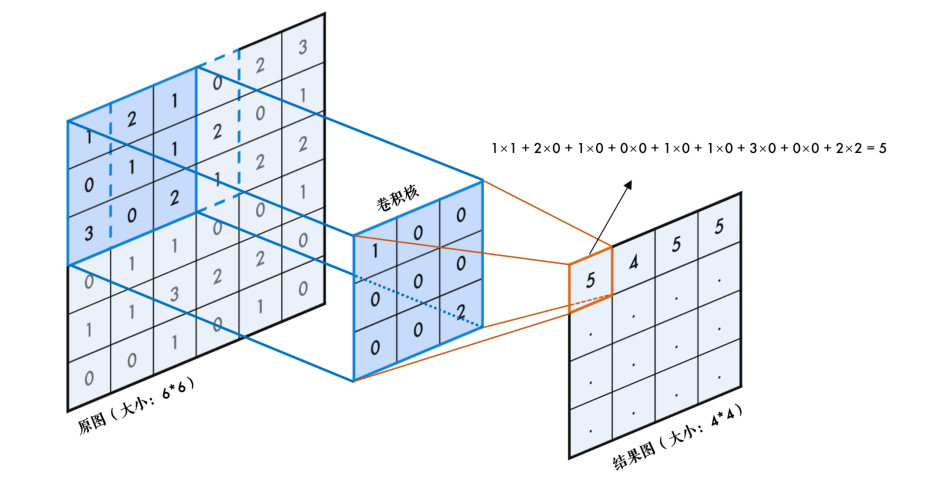
\includegraphics[width=0.7\columnwidth]{pic/con.jpg}
    \caption{一个正在进行的卷积操作示意图\supercite{con}。}
    \label{fig:con}
\end{figure}

一层卷积层便是由N个卷积神经元所组成,每个卷积神经元都有一个$M \times M$的卷积核。因而对于一个输入维度(X,X)的张量,卷积层使用了$N\times M\times M$个参数对输入数据进行处理,输出张量的维度为(N,X-M+1,X-M+1)。而如果试图使用全连接层网络寻找图片的N个特征,那么全连接层的参数数目将会是$N\times X\times X$,远远大于卷积层的参数数目。所以说相对于全连接层,卷积层认为图片的局部特征是有一定的关联性和通用性的,因而可以较小参数的卷积核来表征和卷积操作来表示和提出该特征,从而在大大降低参数数目和计算复杂度的情况下依然拥有着良好的效果。

除了卷积神经网络之外,我们通常还会提到深度神经网络(Deep Neural Network),它的核心便是网络层数多切复杂,网络比较”深“。一般来说,相对于机器学习中的神经网络,拥有两个及以上隐藏层的网络便可以被称作深度神经网络。但是在神经网络中,越是复杂的网络越需要细致的设计和优化调整来达到更为优异的效果,因此在处理具体问题中,相对出从零开始构造一个深度神经网络,尝试和修改既有的深度神经网络更为可行。

递归神经网络(Recurrent Neural Network, RNN)则更适用于处理自然语言识别等相关领域。相对于普通的全连接网络,递归神经网络考虑到了每一层内神经元之间的相互作用,即每次训练中递归层的结果会影响到下一次训练的过程中。因而递归神经网络可以提取数据序列中的相对关系,对于自然语言处理,时间序列数据的处理更为合适。

对抗生成神经网络(Generative Adversarial Network)则是一种特殊的训练网络方式,它使用数据同时训练两个神经网络,一个用于从噪声中生成数据,另一个则鉴别生成器生成的数据,两个网络相互之间不停地对抗,即生成网络试图生成鉴别网络无法区分的数据,而鉴别网络则在努力的识别出由生成网络生成的数据。因而GAN可以从既有的样本中提取信息,并生成类似的数据。

\section{数据准备}
\label{section:data_prepare}

\section{训练网络}
\label{section:train}

\section{测试及结果分析}
\label{section:cnn_result}

% vim:ts=4:sw=4
